\chapter{Limits}
\label{chp:limits}				

\section{Limits}
\label{sec:limits_tutorial}

\marginnote[0.3cm]{The order of the parameters in the \texttt{limit()} command is important. An error message will be displayed if you switch the order of the parameters in the command and then try to execute it.}
We can use the \texttt{limit()} command to evaluate the limit of a function as $x$ approaches $a$. The \texttt{limit()} command needs two parameters. The first parameter is the expression and the second parameter gives the value for a variable to approach.

\begin{maplegroup}
\begin{mapleinput}
\mapleinline{active}{1d}{f(x) := x\symbol{94}2 + 2*x -4;
}{}
\end{mapleinput}
\mapleresult
\begin{maplelatex}
\mapleinline{inert}{2d}{f := proc (x) options operator, arrow; x^2+2*x-4 end proc}{\[\displaystyle f\, := \,x\mapsto {x}^{2}+2\,x-4\]}
\end{maplelatex}
\end{maplegroup}

\begin{maplegroup}
\begin{mapleinput}
\mapleinline{active}{1d}{limit(f(x), x=3);
}{}
\index{limit}
\end{mapleinput}
\mapleresult
\begin{maplelatex}
\mapleinline{inert}{2d}{11}{\[\displaystyle 11\]}
\end{maplelatex}
\end{maplegroup}

\marginnote{It is important to note that $h=0$ here means that $h$ \textit{approaches} $0$, but we are not simply substituting $h=0$ into the expression.}
\begin{maplegroup}
\begin{mapleinput}
\mapleinline{active}{1d}{limit((f(x+h) - f(x))/h, h=0);
}{}
\end{mapleinput}
\mapleresult
\begin{maplelatex}
\mapleinline{inert}{2d}{2x+2}{\[\displaystyle 2x+2\]}
\end{maplelatex}
\end{maplegroup}

\begin{marginfigure}
\centering
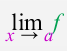
\includegraphics[scale=0.8]{tutorials/figures/palettelimit.png}
\index{limit}
\caption{You can find a shortcut for limits in the palettes toolbar under Calculus.}
\end{marginfigure}

\section{One-Sided Limits}
\label{sec:one_sided_limits}

For one-sided limits, you will need to add an additional parameter to the \texttt{limit()} command, specifying which side (left or right) to approach the value from. In the case of a vertical asymptote, these limits will be equal to $\pm \infty$.

\begin{maplegroup}
\begin{mapleinput}
\mapleinline{active}{1d}{L(x) := 1/x;
}{}
\end{mapleinput}
\mapleresult
\begin{maplelatex}
\mapleinline{inert}{2d}{L := proc (x) options operator, arrow; 1/x end proc}{\[\displaystyle L\, := \,x\mapsto {x}^{-1}\]}
\end{maplelatex}
\end{maplegroup}

\marginnote[0.5cm]{Some versions of Maple may not properly display graphs of functions that contain vertical asymptotes. Include \texttt{discont=true} as a parameter in the \texttt{plot( )} command when required. \index{plot!discontinuities}}
\begin{maplegroup}
\begin{mapleinput}
\mapleinline{active}{1d}{plot(L(x), x=-3..3, y=-5..5);
}{}
\end{mapleinput}
\mapleresult
\mapleplot{tutorials/figures/Limitsplot2d1-eps-converted-to.pdf}
\end{maplegroup}

\begin{maplegroup}
\begin{mapleinput}
\mapleinline{active}{1d}{limit(L(x), x=0, right);
}{}
\index{limit!one-sided}
\end{mapleinput}
\mapleresult
\begin{maplelatex}
\mapleinline{inert}{2d}{infinity}{\[\displaystyle \infty \]}
\end{maplelatex}
\end{maplegroup}

\begin{maplegroup}
\begin{mapleinput}
\mapleinline{active}{1d}{limit(L(x), x=0, left);
}{}
\index{limit!one-sided}
\end{mapleinput}
\mapleresult
\begin{maplelatex}
\mapleinline{inert}{2d}{-infinity}{\[\displaystyle -\infty \]}
\end{maplelatex}
\end{maplegroup}

\begin{maplegroup}
\begin{mapleinput}
\mapleinline{active}{2d}{}{\[\]}
\end{mapleinput}
\end{maplegroup}

\subsection{Vertical Asymptotes and One-Sided Limits}
\label{subsec:vertical_asymptotes}

In this example, we will examine a rational function and use limits to determine its vertical asymptotes.

\begin{maplegroup}
\begin{mapleinput}
\mapleinline{active}{1d}{f(x) := (x\symbol{94}2-x-6)/(x\symbol{94}2-8*x+15);
}{}
\end{mapleinput}
\mapleresult
\begin{maplelatex}
\mapleinline{inert}{2d}{f := proc (x) options operator, arrow; (x^2-x-6)/(x^2-8*x+15) end proc}{\[\displaystyle f\, := \,x\mapsto {\frac {{x}^{2}-x-6}{{x}^{2}-8\,x+15}}\]}
\end{maplelatex}
\end{maplegroup}

\noindent
We can factor the denominator to find the domain of $f(x)$ and predict where we might find vertical asymptotes.

\marginnote{There is a useful \texttt{denom()}\index{mathematical functions!denominator} command that Maple provides. You can type \texttt{denom(f(x))} to get the denominator of $f(x)$.}
\begin{maplegroup}
\begin{mapleinput}
\mapleinline{active}{1d}{factor(x\symbol{94}2-8*x+15);
}{}
\end{mapleinput}
\mapleresult
\begin{maplelatex}
\mapleinline{inert}{2d}{(x-3)*(x-5)}{\[\displaystyle  \left( x-3 \right)  \left( x-5 \right) \]}
\end{maplelatex}
\end{maplegroup}

\noindent
It looks like $x=3$ and $x=5$ are not in the domain of $f(x)$. We can find the limit of $f(x)$ as $x \rightarrow 3$.

\begin{maplegroup}
\begin{mapleinput}
\mapleinline{active}{1d}{limit(f(x), x=3);
}{}
\end{mapleinput}
\mapleresult
\begin{maplelatex}
\mapleinline{inert}{2d}{-5/2}{\[\displaystyle -5/2\]}
\end{maplelatex}
\end{maplegroup}

\noindent
Since this limit exists but $f(3)$ does not, this is a \textit{removable discontinuity} and not a vertical asymptote. Now we can find the limit of $f(x)$ as $x \rightarrow 5$.

\begin{maplegroup}
\begin{mapleinput}
\mapleinline{active}{1d}{limit(f(x), x=5);
}{}
\end{mapleinput}
\mapleresult
\begin{maplelatex}
\mapleinline{inert}{2d}{undefined}{\[\displaystyle {\it undefined}\]}
\end{maplelatex}
\end{maplegroup}

\noindent
Even though this limit does not exist, we cannot automatically conclude that $f(x)$ has a vertical asymptote at $x=5$. We need to compute the one-sided limits to see if there is asymptotic behaviour.

\marginnote{Maple provides an \texttt{Asymptotes()} command that you can investigate using Maple help. Try typing \texttt{?Asymptotes} to learn more.}
\begin{maplegroup}
\begin{mapleinput}
\mapleinline{active}{1d}{limit(f(x), x=5, left);
}{}
\end{mapleinput}
\begin{mapleinput}
\mapleinline{active}{1d}{limit(f(x), x=5, right);
}{}
\end{mapleinput}
\mapleresult
\begin{maplelatex}
\mapleinline{inert}{2d}{-infinity}{\[\displaystyle -\infty \]}
\end{maplelatex}
\mapleresult
\begin{maplelatex}
\mapleinline{inert}{2d}{infinity}{\[\displaystyle \infty \]}
\end{maplelatex}
\end{maplegroup}

\noindent
Since these limits are given as $\pm \infty$, we know that $f(x)$ has a vertical asymptote at $x=5$.

\section{Limits at Infinity}
\label{sec:limits_at_infinity}

To take the limit of a function as $x$ becomes infinitely large, Maple recognizes \texttt{infinity} and \texttt{-infinity}. These can be used to find horizontal asymptotes. If the function does not have a horizontal asymptote, the limit may result in $\pm \infty$.

\begin{maplegroup}
\begin{mapleinput}
\mapleinline{active}{1d}{g(x) := (3*x\symbol{94}2 + 5*x - 10) / (5*x\symbol{94}2 - 20*x + 1);
}{}
\end{mapleinput}
\mapleresult
\begin{maplelatex}
\mapleinline{inert}{2d}{g := proc (x) options operator, arrow; (3*x^2+5*x-10)/(5*x^2-20*x+1) end proc}{\[\displaystyle g\, := \,x\mapsto {\frac {3\,{x}^{2}+5\,x-10}{5\,{x}^{2}-20\,x+1}}\]}
\end{maplelatex}
\end{maplegroup}
\index{limit!at infinity}
\begin{maplegroup}
\begin{mapleinput}
\mapleinline{active}{1d}{limit(g(x), x=infinity);
}{}
\end{mapleinput}
\mapleresult
\begin{maplelatex}
\mapleinline{inert}{2d}{3/5}{\[\displaystyle 3/5\]}
\end{maplelatex}
\end{maplegroup}

\begin{maplegroup}
\begin{mapleinput}
\mapleinline{active}{2d}{}{\[\]}
\end{mapleinput}
\end{maplegroup}

An oscillating function such as $\sin(x)$ may not have a definable limit. Maple will attempt to determine a range for the minimum and maximum of the function.

\begin{maplegroup}
\begin{mapleinput}
\mapleinline{active}{1d}{h(x) := sin(x);
}{}
\end{mapleinput}
\mapleresult
\begin{maplelatex}
\mapleinline{inert}{2d}{h := proc (x) options operator, arrow; sin(x) end proc}{\[\displaystyle h\, := \,x\mapsto \sin \left( x \right) \]}
\end{maplelatex}
\end{maplegroup}

\marginnote{Since $\sin(x)$ oscillates between $-1$ and $1$, Maple cannot determine a unique value for the limit as $x \rightarrow -\infty$.}
\begin{maplegroup}
\begin{mapleinput}
\mapleinline{active}{1d}{limit(h(x), x=-infinity);
}{}
\index{limit!at infinity}
\end{mapleinput}
\mapleresult
\begin{maplelatex}
\mapleinline{inert}{2d}{-1 .. 1}{\[\displaystyle {-1\ldots 1}\]}
\end{maplelatex}
\end{maplegroup}

\subsection{Horizontal Asymptotes and Limits at Infinity}
\label{subsec:horizontal_asymptotes}

In this example, we will examine the function
\[ f(t) = \frac{2000}{1+{\rm e}^{-t+2}}, \]
which is known as a logistic function.
\index{mathematical functions!logistic function}
\index{mathematical functions!exponential function}
\index{plot}
\begin{maplegroup}
\begin{mapleinput}
\mapleinline{active}{1d}{logistic(t) := 2000/(1 + exp(-t+2));
}{}
\end{mapleinput}
\mapleresult
\begin{maplelatex}
\mapleinline{inert}{2d}{logistic := proc (t) options operator, arrow; 2000/(1+exp(-t+2)) end proc}{\[\displaystyle {\it logistic}\, := \,t\mapsto \frac{2000}{1+{{\rm e}^{-t+2}}}\]}
\end{maplelatex}
\end{maplegroup}

\noindent
Judging by the plot of the logistic function, it appears that the function may have horizontal asymptotes.

\marginnote{Logistic functions have many applications, such as population modeling.}
\begin{maplegroup}
\begin{mapleinput}
\mapleinline{active}{1d}{plot(logistic(t));}{}
\end{mapleinput}
\mapleresult
\mapleplot{tutorials/figures/logisticasymptotesplot2d1-eps-converted-to.pdf}
\end{maplegroup}

To find the right-hand asymptote, we take the limit as $t \rightarrow \infty$.
\marginnote{Here we are using \texttt{t=infinity} rather than $x$, since the variable of this function is $t$.}

\begin{maplegroup}
\begin{mapleinput}
\mapleinline{active}{1d}{limit(logistic(t), t=infinity);
}{}
\end{mapleinput}
\mapleresult
\begin{maplelatex}
\mapleinline{inert}{2d}{2000}{\[\displaystyle 2000\]}
\end{maplelatex}
\end{maplegroup}

To find the left-hand asymptote, we take the limit as $t \rightarrow -\infty$.

\begin{maplegroup}
\begin{mapleinput}
\mapleinline{active}{1d}{limit(logistic(t), t=-infinity);
}{}
\end{mapleinput}
\mapleresult
\begin{maplelatex}
\mapleinline{inert}{2d}{0}{\[\displaystyle 0\]}
\end{maplelatex}
\end{maplegroup}

\section{Limits and Piecewise Functions}
\label{sec:limits_and_piecewise_functions}

A piecewise function is a good opportunity to practice plotting discontinuities and investigating one- and two-sided limits.
\index{mathematical functions!piecewise}
\begin{maplegroup}
\begin{mapleinput}
\mapleinline{active}{1d}{P(x) := piecewise(x<=-1, x\symbol{94}2, x<=1, -x, 1<x, x-4);
}{}
\end{mapleinput}
\mapleresult
\begin{maplelatex}
\mapleinline{inert}{2d}{P := proc (x) options operator, arrow; piecewise(x <= -1, x^2, x <= 1, -x, 1 < x, x-4) end proc}{\[\displaystyle P\, := \,x\mapsto \begin{cases}{x}^{2}&x\leq -1 \\ -x&x\leq 1 \\ x-4&1<x\end{cases}\]}
\end{maplelatex}
\end{maplegroup}

\begin{maplegroup}
\begin{mapleinput}
\mapleinline{active}{1d}{P(x);
}{}
\end{mapleinput}
\mapleresult
\begin{maplelatex}
\mapleinline{inert}{2d}{piecewise(x <= -1, x^2, x <= 1, -x, 1 < x, x-4)}{\[\displaystyle \begin{cases}{x}^{2}& x\leq -1 \\ -x& x\leq 1 \\ x-4&1<x\end{cases}\]}
\end{maplelatex}
\end{maplegroup}
\marginnote[.3cm]{It is necessary to include the \texttt{discont=true} parameter in the \texttt{plot(~)} command here so that the jump discontinuity is properly displayed in the graph of this piecewise function.}
\marginnote[1cm]{Unfortunately, even with the \texttt{discont=true} option, Maple does not include an open dot at $(1,-3)$.}
\begin{maplegroup}
\begin{mapleinput}
\mapleinline{active}{1d}{plot(P(x), x=-4..4, y=-5..5, discont=true);
}{}
\end{mapleinput}
\mapleresult
\mapleplot{tutorials/figures/Limitsplot2d2-eps-converted-to.pdf}
\end{maplegroup}
\index{plot}
 \index{plot!discontinuities}
\index{limit}
\index{limit!one-sided}
\begin{maplegroup}
\begin{mapleinput}
\mapleinline{active}{1d}{limit(P(x), x=1);
}{}
\end{mapleinput}
\mapleresult
\begin{maplelatex}
\mapleinline{inert}{2d}{undefined}{\[\displaystyle {\it undefined}\]}
\end{maplelatex}
\end{maplegroup}

\begin{maplegroup}
\begin{mapleinput}
\mapleinline{active}{1d}{limit(P(x), x=1, left);
}{}
\end{mapleinput}
\mapleresult
\begin{maplelatex}
\mapleinline{inert}{2d}{-1}{\[\displaystyle -1\]}
\end{maplelatex}
\end{maplegroup}

\begin{maplegroup}
\begin{mapleinput}
\mapleinline{active}{1d}{limit(P(x), x=1, right);
}{}
\end{mapleinput}
\mapleresult
\begin{maplelatex}
\mapleinline{inert}{2d}{-3}{\[\displaystyle -3\]}
\end{maplelatex}
\end{maplegroup}

\section{The Limit Methods Tutor}\index{limit!tutor}
\label{sec:limitmethodstutor}

The Limit Methods tutor will walk you through each step needed to evaluate a limit, including all of the limit laws learned in class. The tutor will open in a new interactive window and will output all steps in your Maple worksheet once the window is closed.

\begin{figure}[h]
\caption{Opening up the Limit Methods tutor using menus.}
\centering
\adjincludegraphics[width=\textwidth]{tutorials/figures/LimitTutorLoad-eps-converted-to.pdf}
\end{figure}

\begin{figure}[h]
\caption{Opening up the Limit Methods tutor using commands. The \texttt{Student[Calculus1]} package is required.}
\centering
\adjincludegraphics[width=\textwidth]{tutorials/figures/LimitTutorLoad2-eps-converted-to.pdf}
\end{figure}

\newpage

\subsection{Using Limit Laws for a One-sided Limit}

\index{limit!tutor!one-sided}
This example will illustrate all of the steps required to evaluate \[ \displaystyle\lim_{x \rightarrow 2^+} \frac{x-2}{x^2-x-2}. \]
\begin{figure}[h]
\caption{Begin by typing out the function, the variable name, and the value that you want the variable to approach. The direction can be specified in the drop down menu to the right of the variable information. Hit Start. You can click on individual limit laws to see whether they apply to the given limit.}
\centering
\adjincludegraphics[width=0.9\textwidth,trim={0 {0.2\height} 0 0},clip]{tutorials/figures/LimitTutorQ1-1-eps-converted-to.pdf}
\vspace{-1cm}
\end{figure}
\marginnote[-2.9cm]{When typing out the function in the tutor, you will not have access to the palettes toolbar in Maple. You will need to type out commands such as \texttt{sqrt()} for square roots. You must also include the symbol * for multiplication.}

\begin{figure}[h]
\caption{You can press the Next Step or All Steps buttons to have Maple show you a step-by-step solution.}
\centering
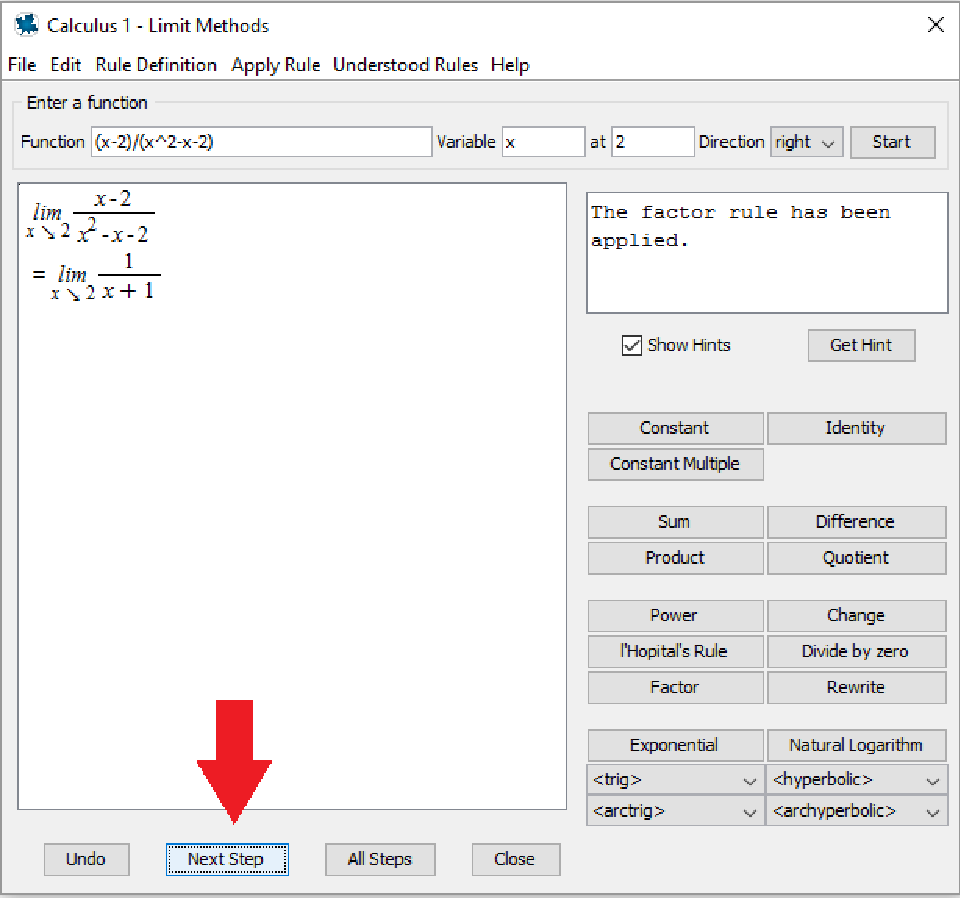
\includegraphics[width=0.9\textwidth]{tutorials/figures/LimitTutorQ1-2-eps-converted-to.pdf}
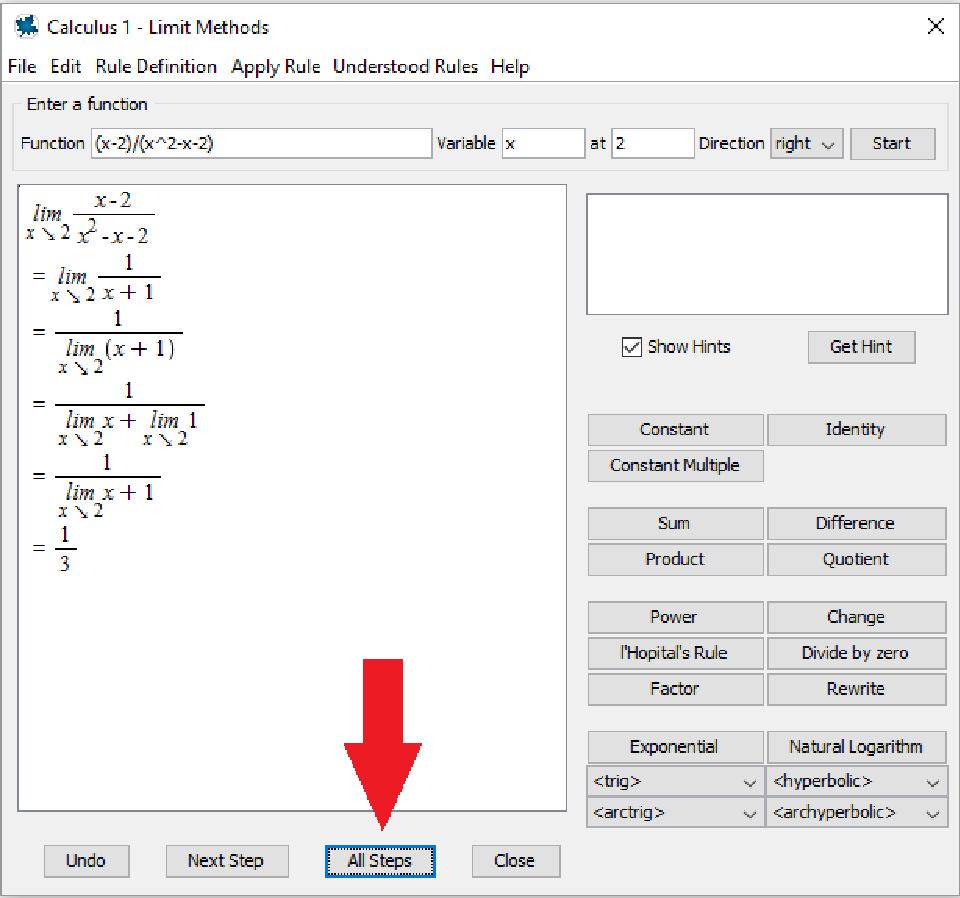
\includegraphics[width=0.9\textwidth]{tutorials/figures/LimitTutorQ1-3-eps-converted-to.pdf}
\end{figure}
\newpage

\clearpage

\subsection{Using Limit Laws for a Limit at Infinity}

\index{limit!tutor!at infinity}
In this example, we will see all of the limit laws used to evaluate \[ \displaystyle\lim_{x \rightarrow -\infty} \frac{2x-1}{\sqrt{x^2-x+3}}. \]

\begin{figure}[h]
\caption{For a limit as $x \rightarrow \infty$ or $x \rightarrow -\infty$, Maple recognizes the word \texttt{infinity}.}
\centering
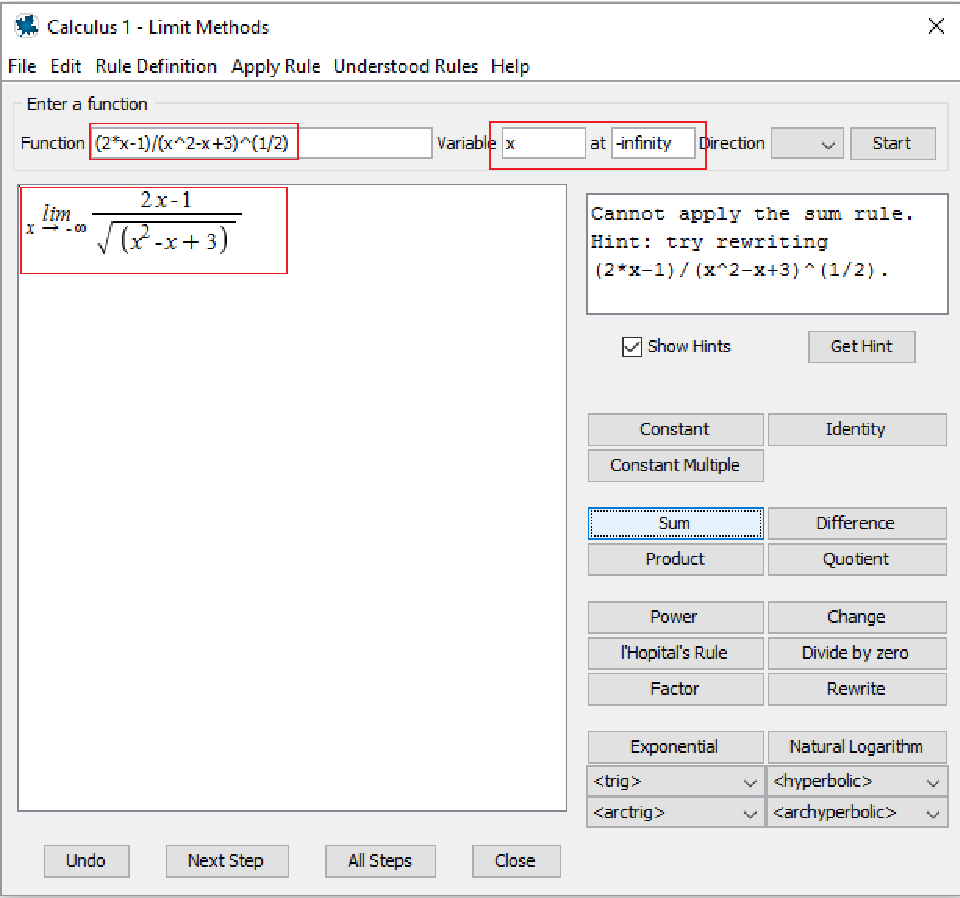
\includegraphics[width=\textwidth]{tutorials/figures/LimitTutorQ2-1-eps-converted-to.pdf}
\end{figure}
\marginnote[-3cm]{An alternate method for inputting the function into the tutor involves the \texttt{sqrt()} command.}

\begin{figure}[h]
\caption{You can click the Next Step or All Steps buttons to have Maple show you a step-by-step solution.}
\centering
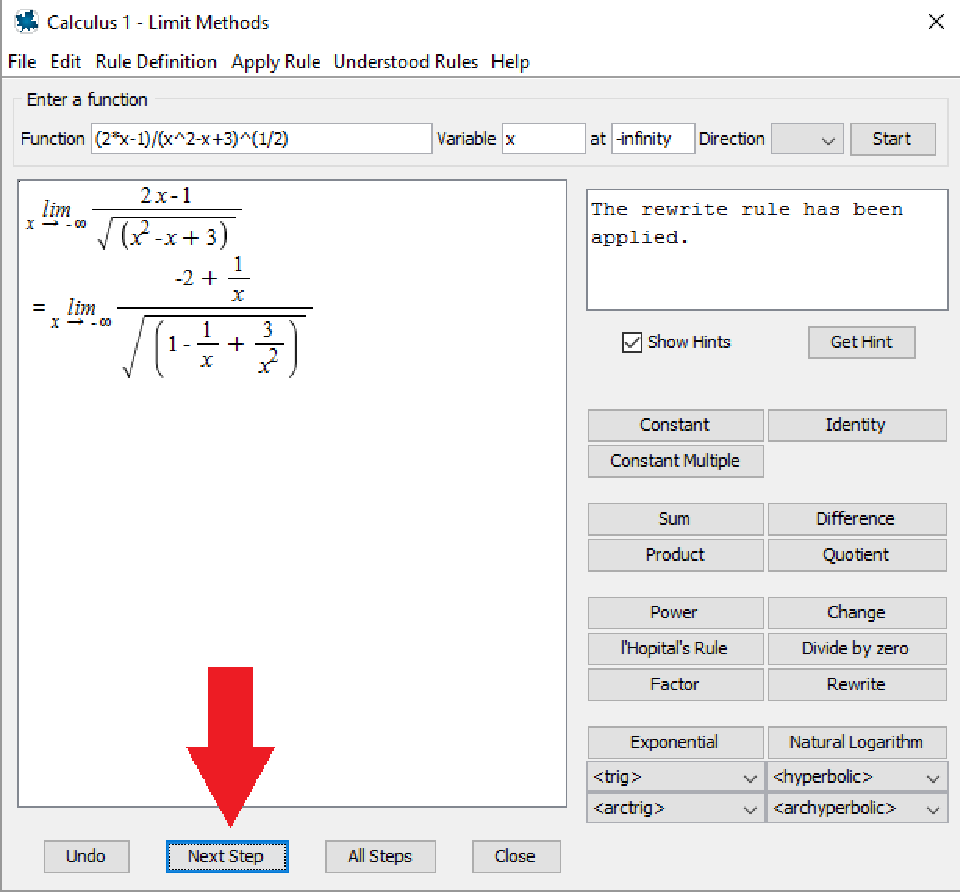
\includegraphics[width=\textwidth]{tutorials/figures/LimitTutorQ2-2-eps-converted-to.pdf}
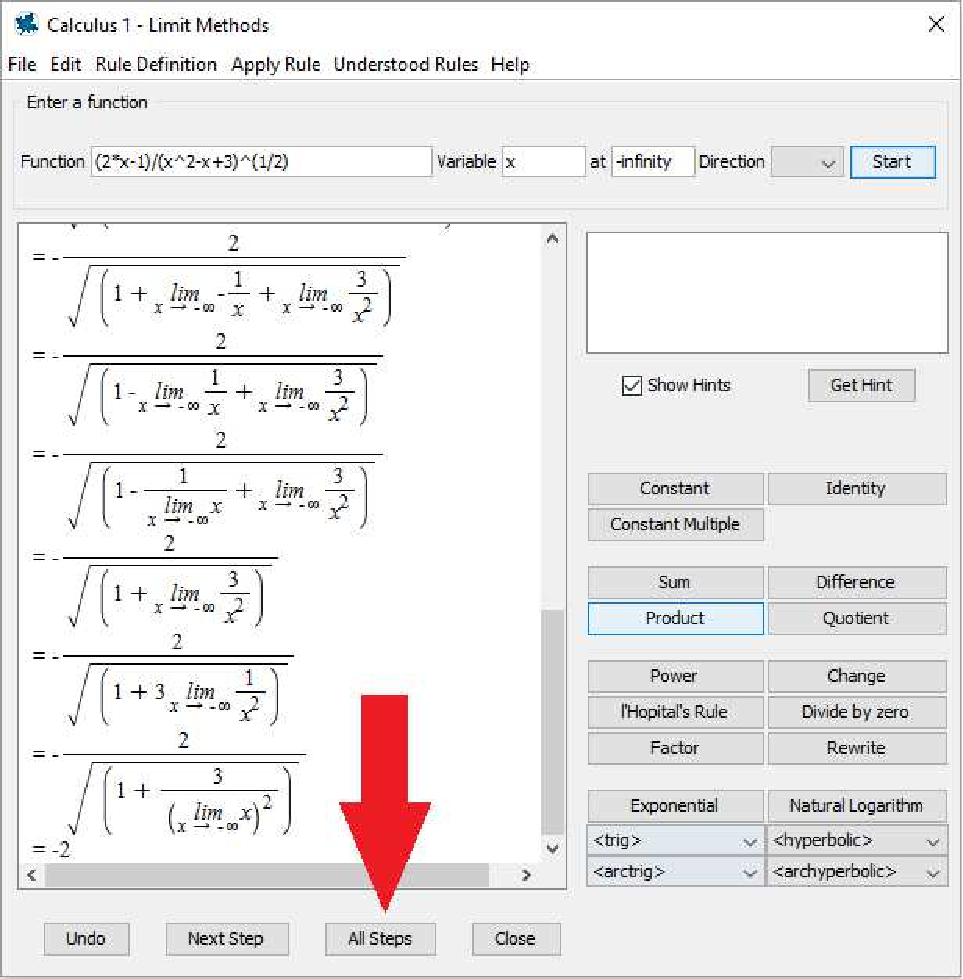
\includegraphics[width=\textwidth]{tutorials/figures/LimitTutorQ2-3-eps-converted-to.pdf}
\end{figure}